\subsubsection{Giao diện Admin - Quản lý công ty}

Tương tự trang quản lý công việc, trang quản lý công ty cũng sử dụng các loại truy vấn sau để hỗ trợ cho các thao tác CRUD:
\begin{itemize}
    \item \textbf{Query with single/composite condition}: Để fetch lên dữ liệu toàn bộ công ty trong hệ thống theo cơ chế phân trang và một số điều kiện như \textbf{Tên công ty}, \textbf{Địa chỉ}
    \begin{figure}[H]
        \centering
        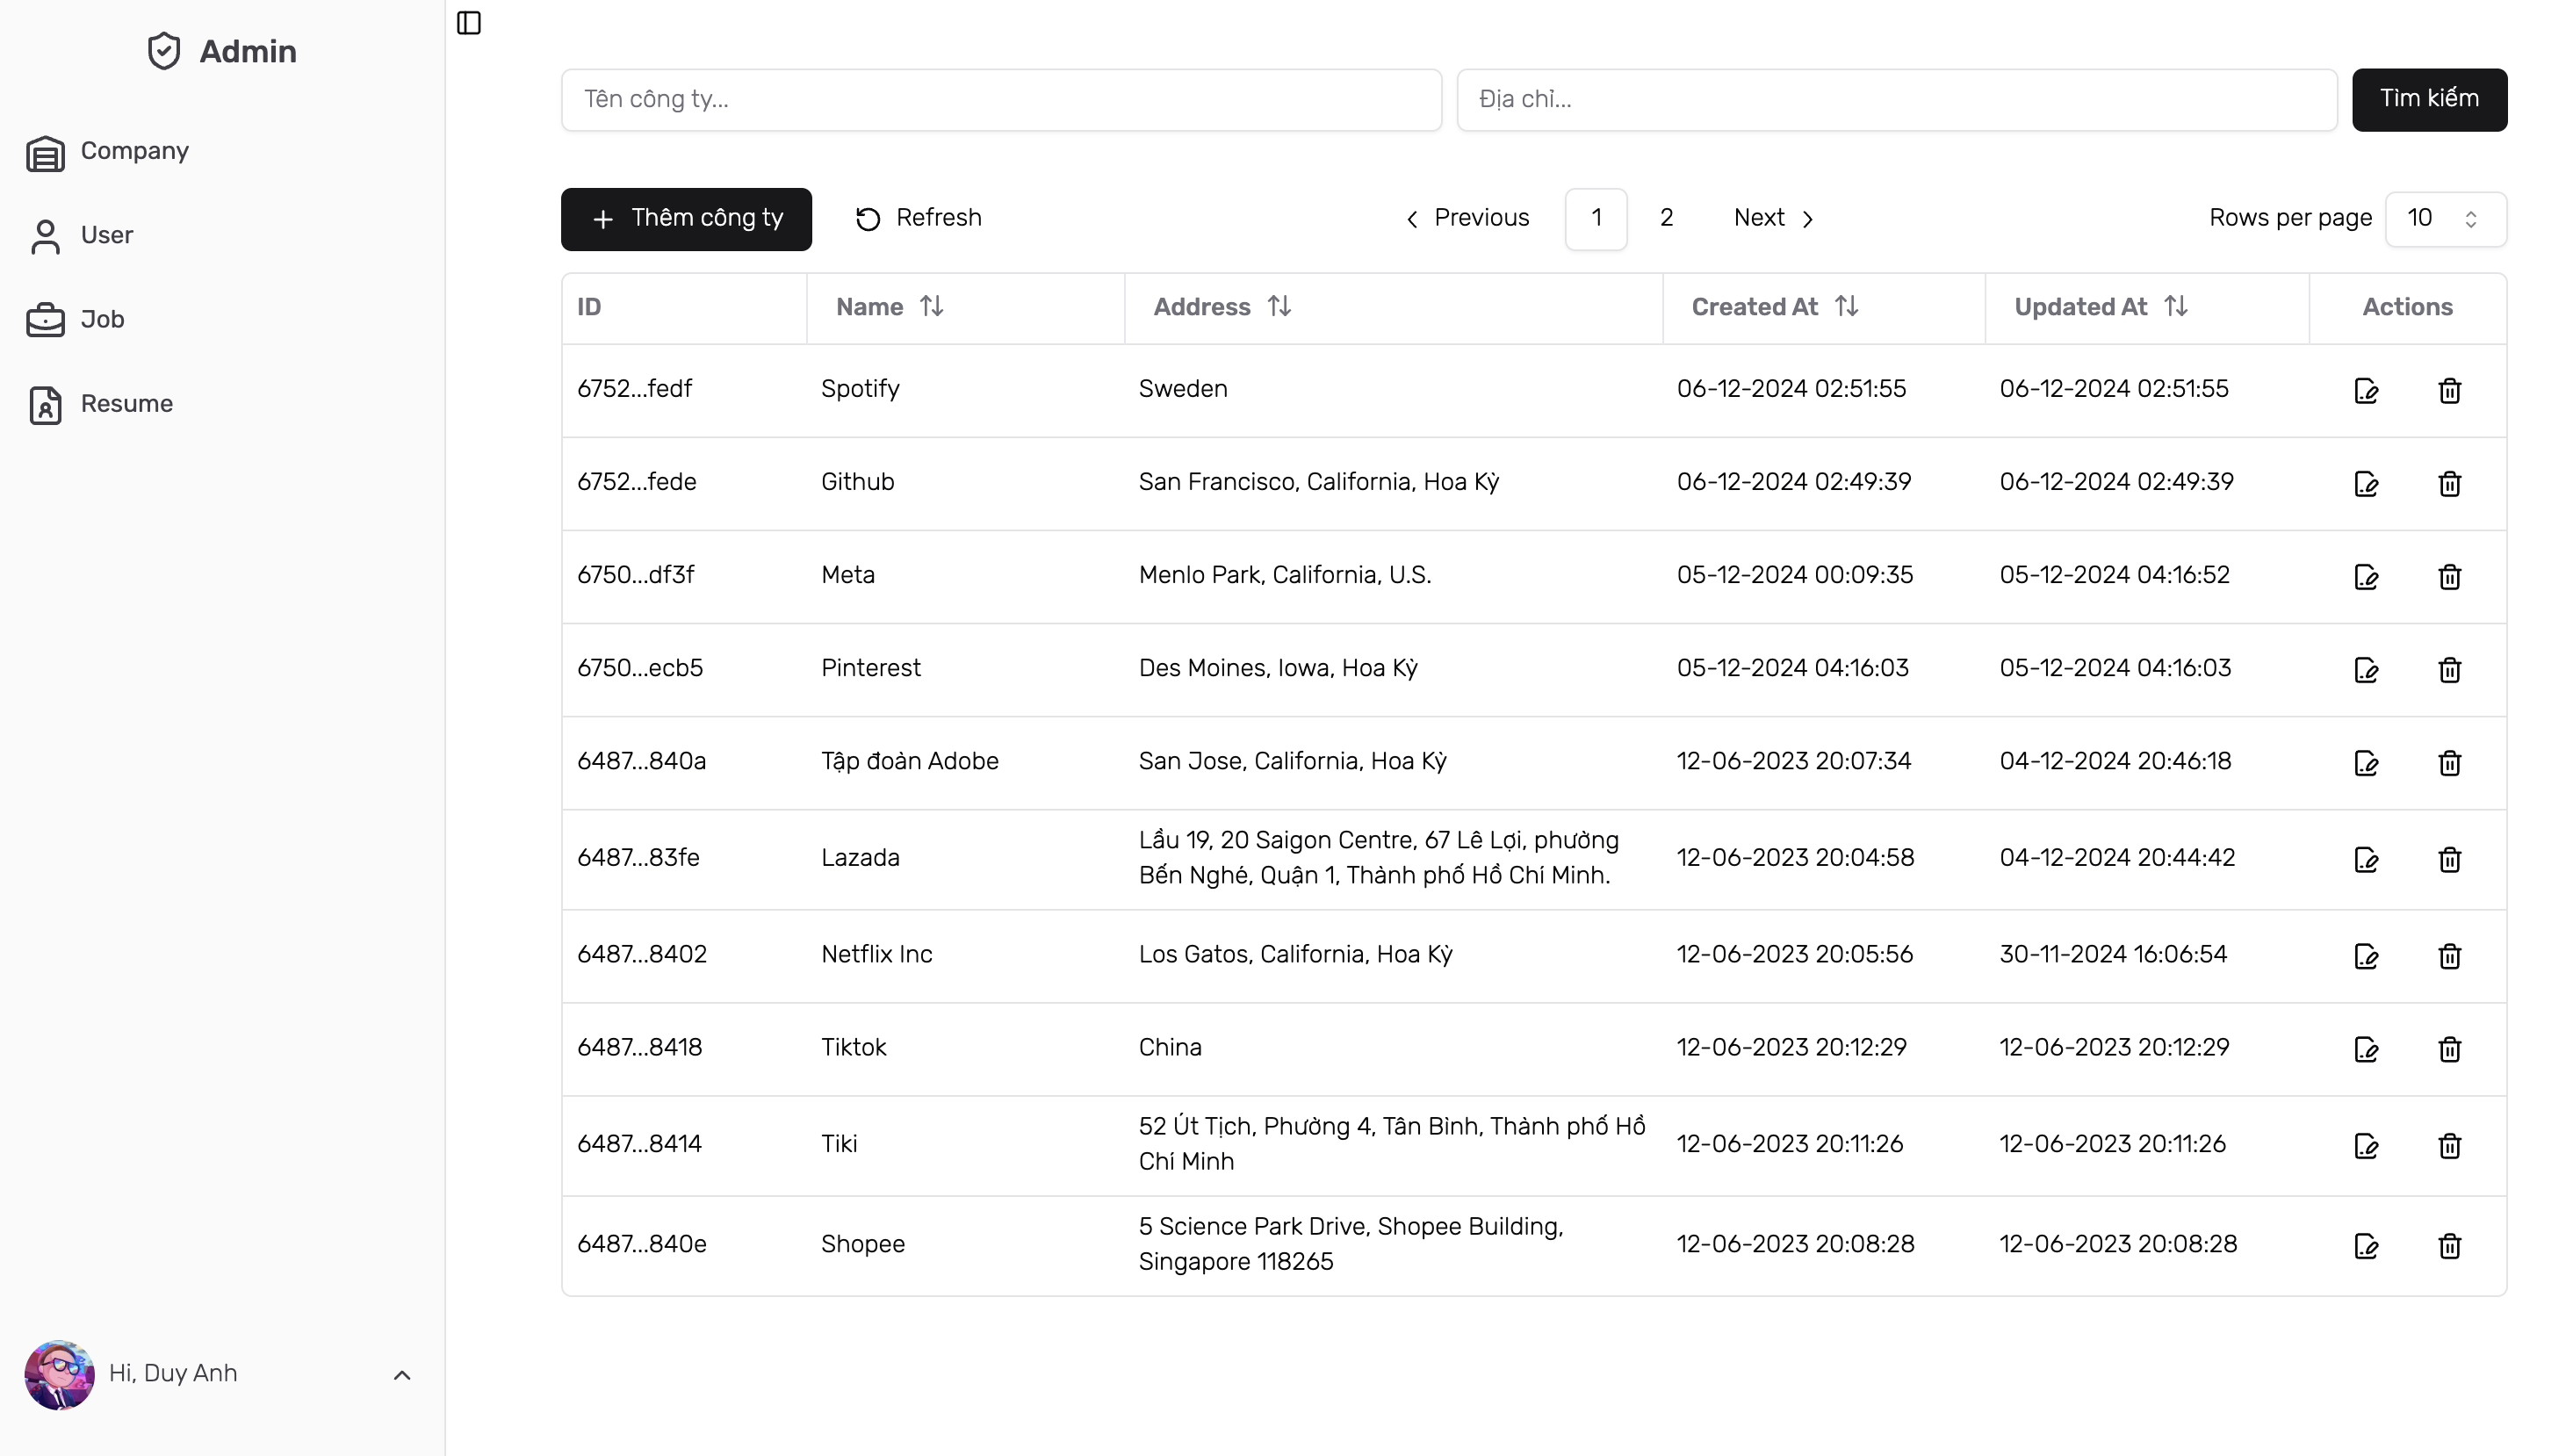
\includegraphics[width=\linewidth]{DBMS-Application/Images/admin-company.png}
        \caption{Trang quản lý công ty - Danh sách các công ty trong hệ thống}
        \label{fig:enter-label}
    \end{figure}

    \begin{figure}[H]
        \centering
        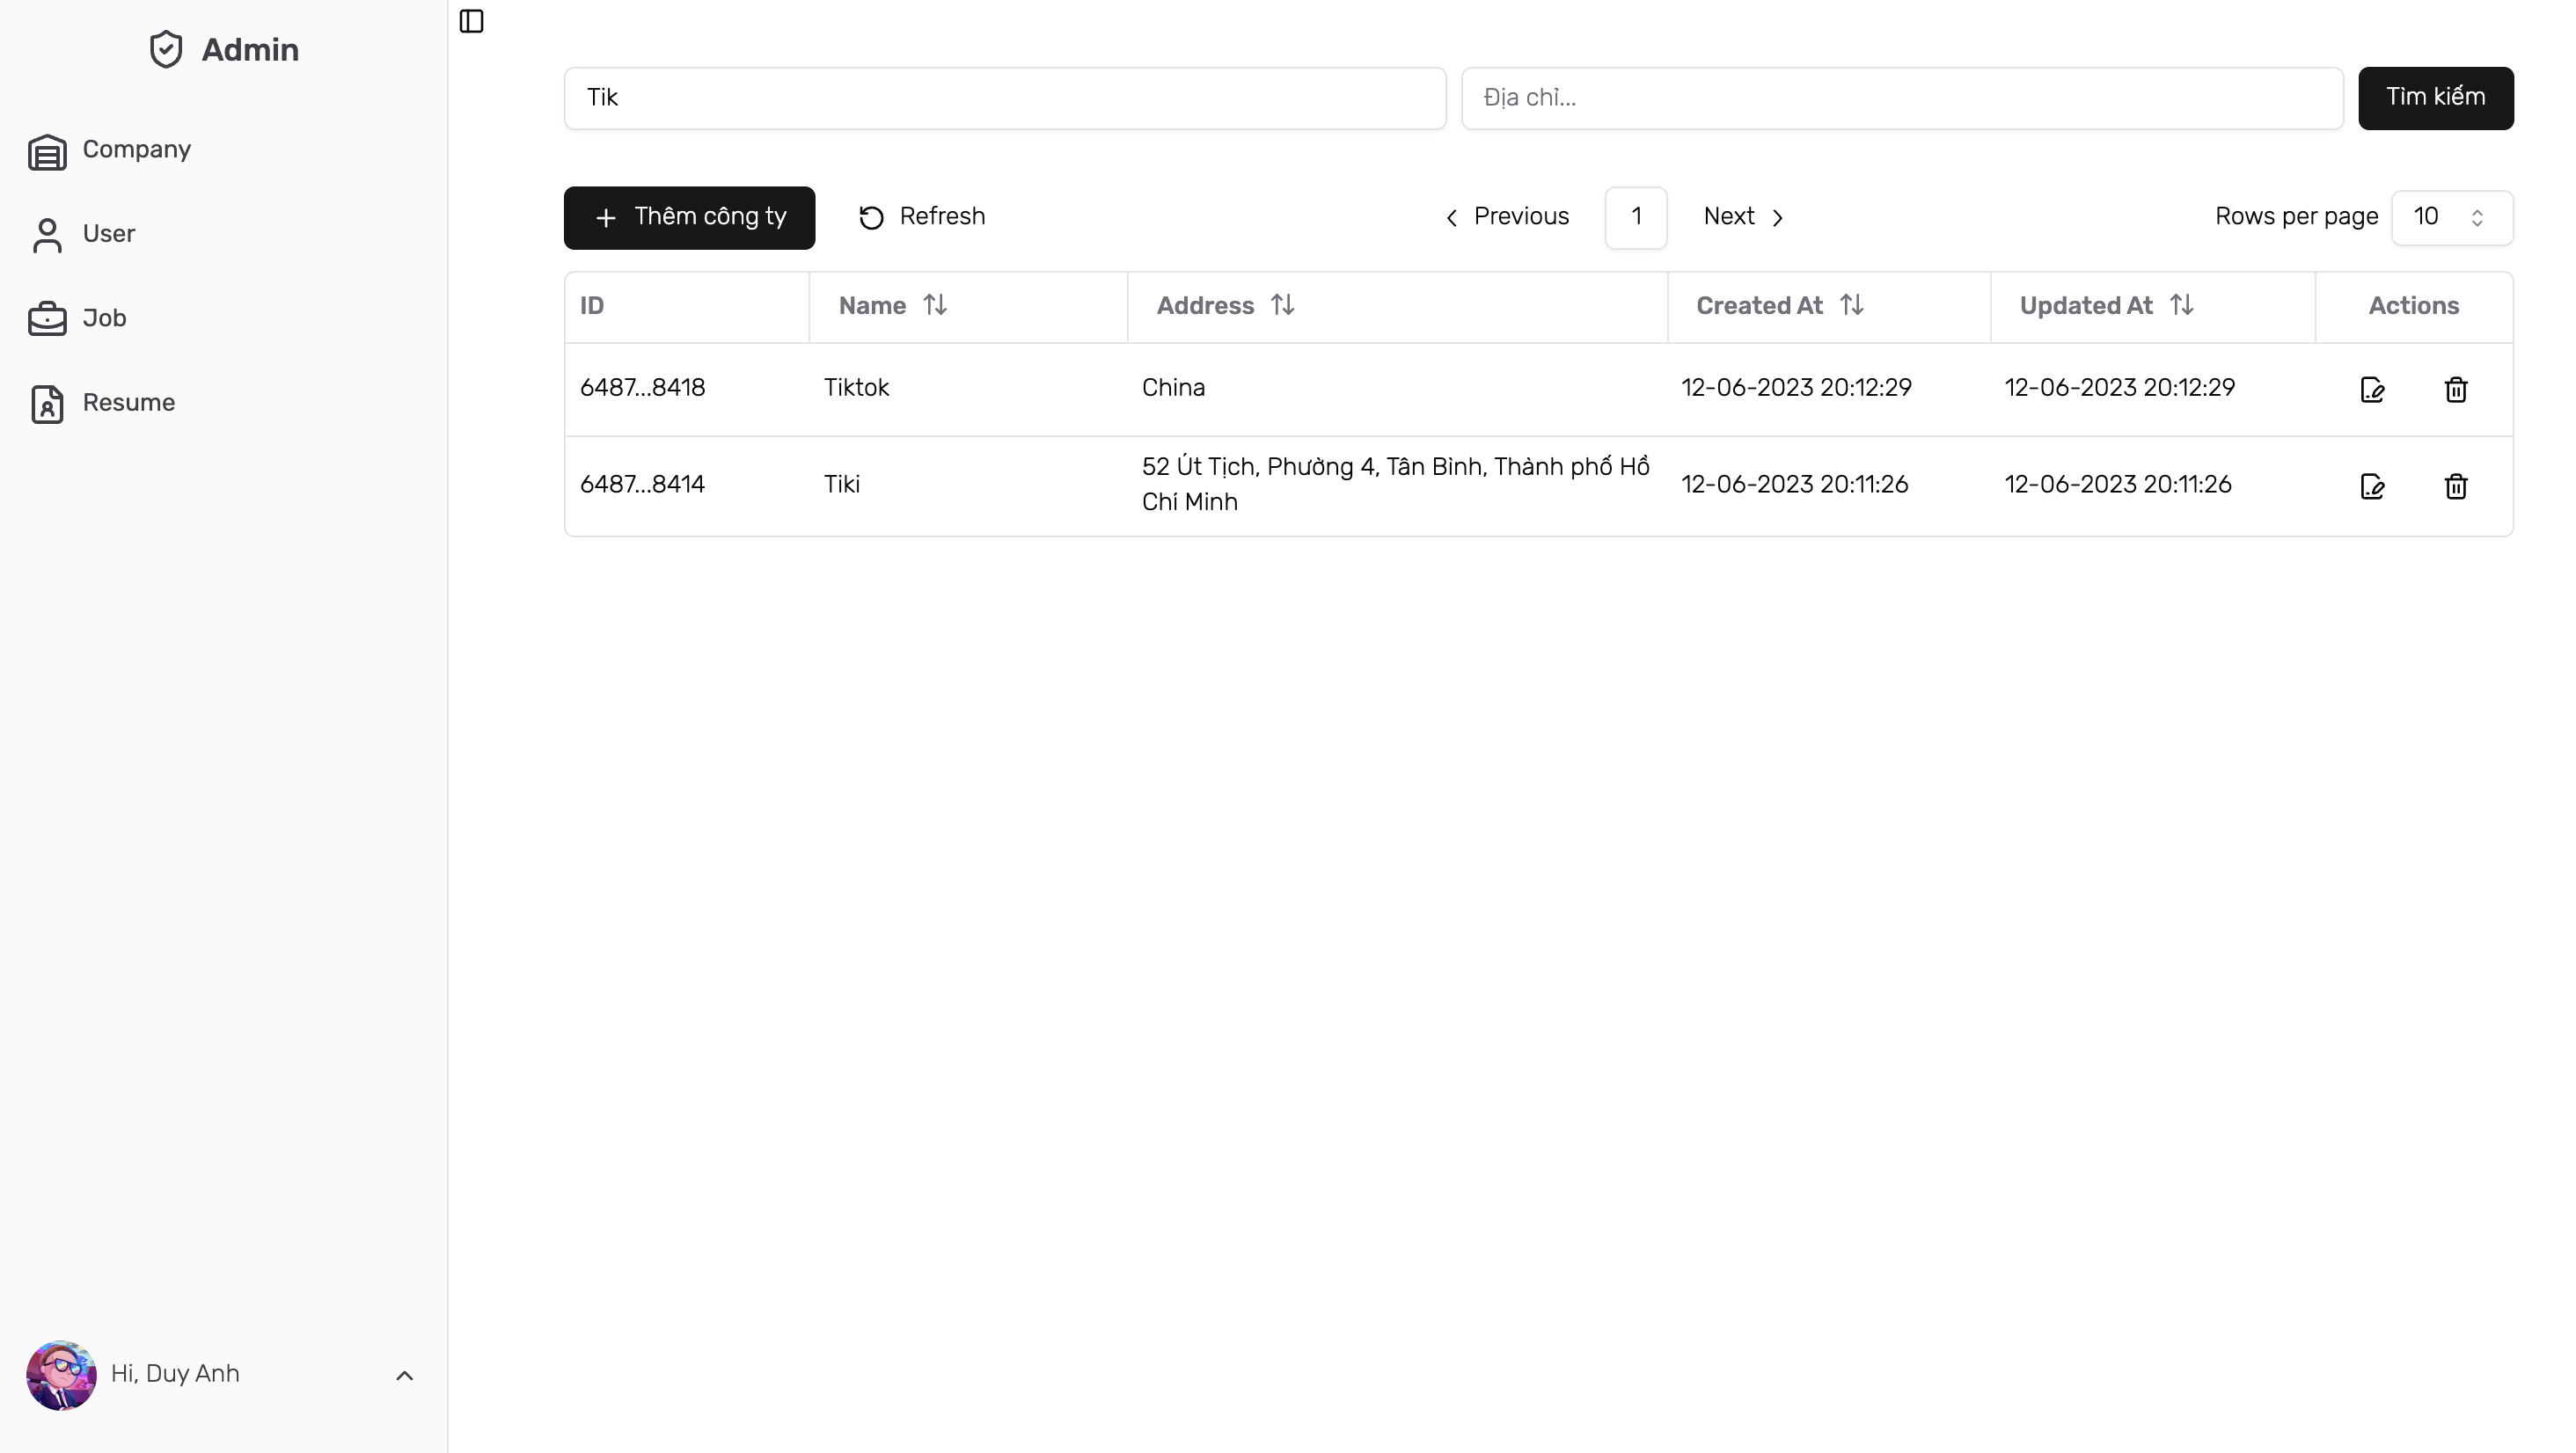
\includegraphics[width=\linewidth]{DBMS-Application/Images/admin-company-filter.png}
        \caption{Trang quản lý công ty - Danh sách công ty lọc theo điều kiện}
        \label{fig:enter-label}
    \end{figure}
    
    \item \textbf{Insert}: Thêm mới một công ty
    \begin{figure}[H]
        \centering
        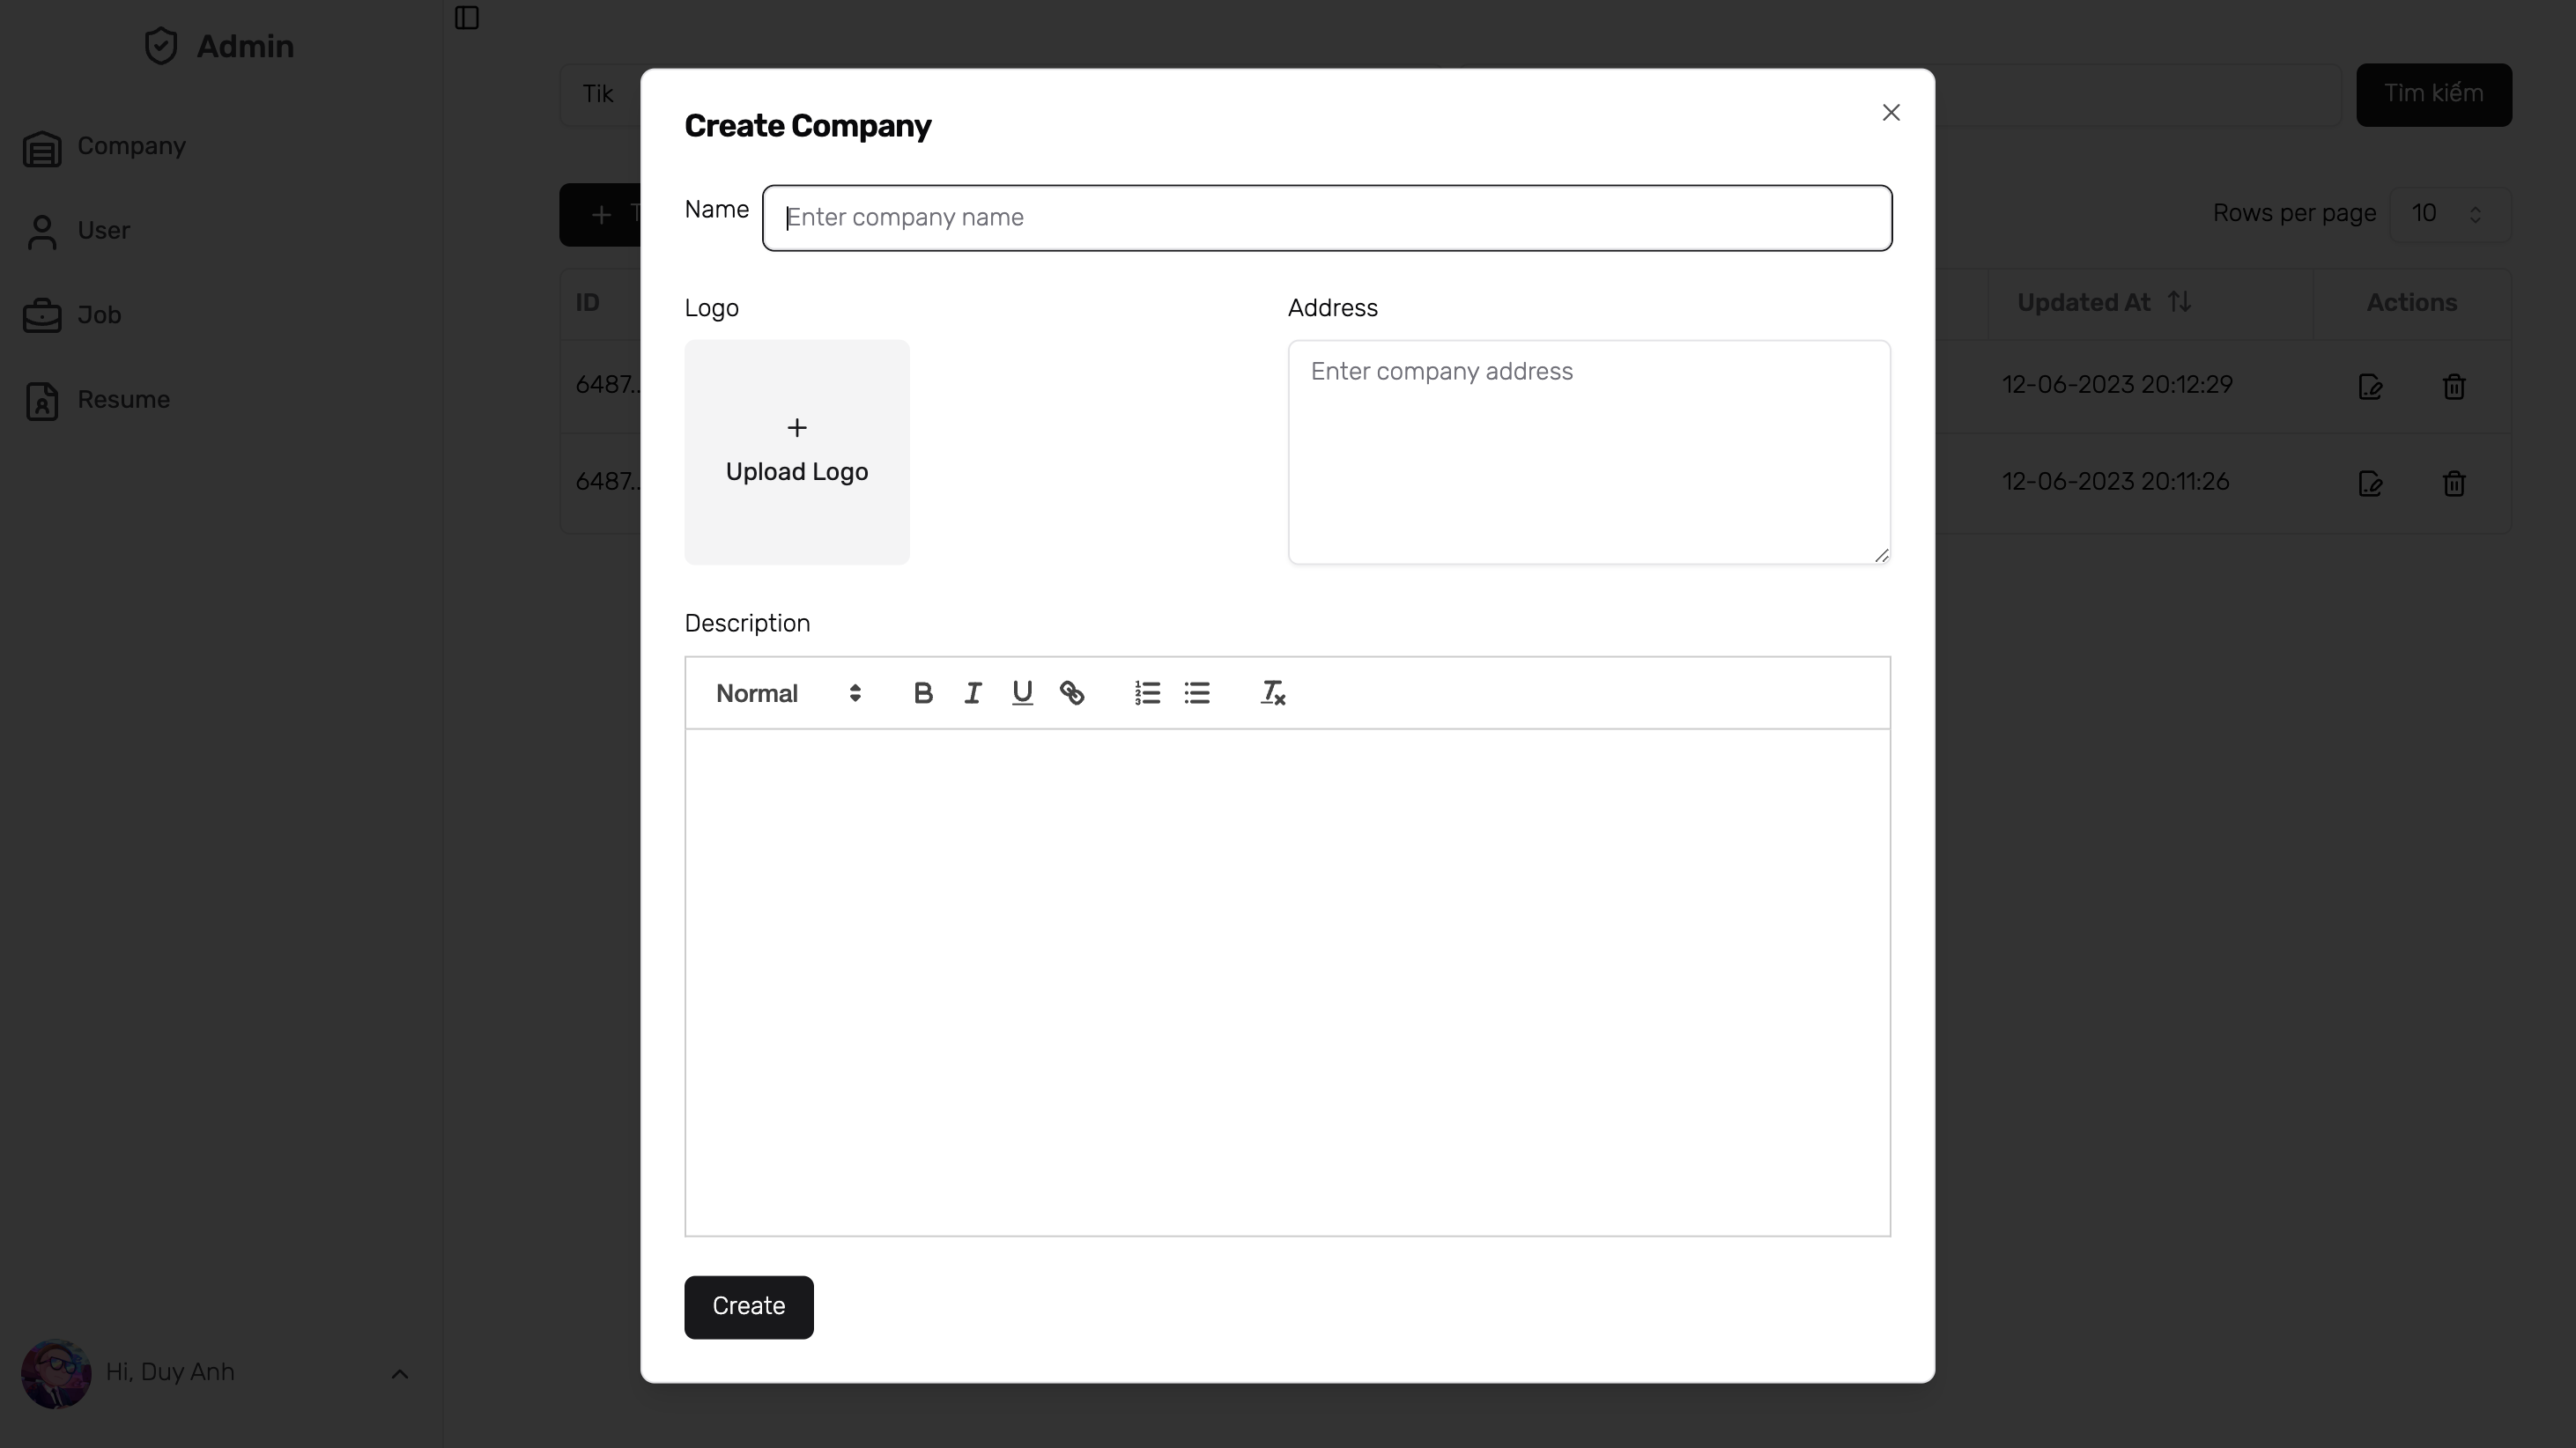
\includegraphics[width=\linewidth]{DBMS-Application/Images/create-company.png}
        \caption{Trang quản lý công ty - Thêm mới công ty}
        \label{fig:enter-label}
    \end{figure}

    \item \textbf{Update}: Cập nhật/chỉnh sửa thông tin công ty cụ thể
    \begin{figure}[H]
        \centering
        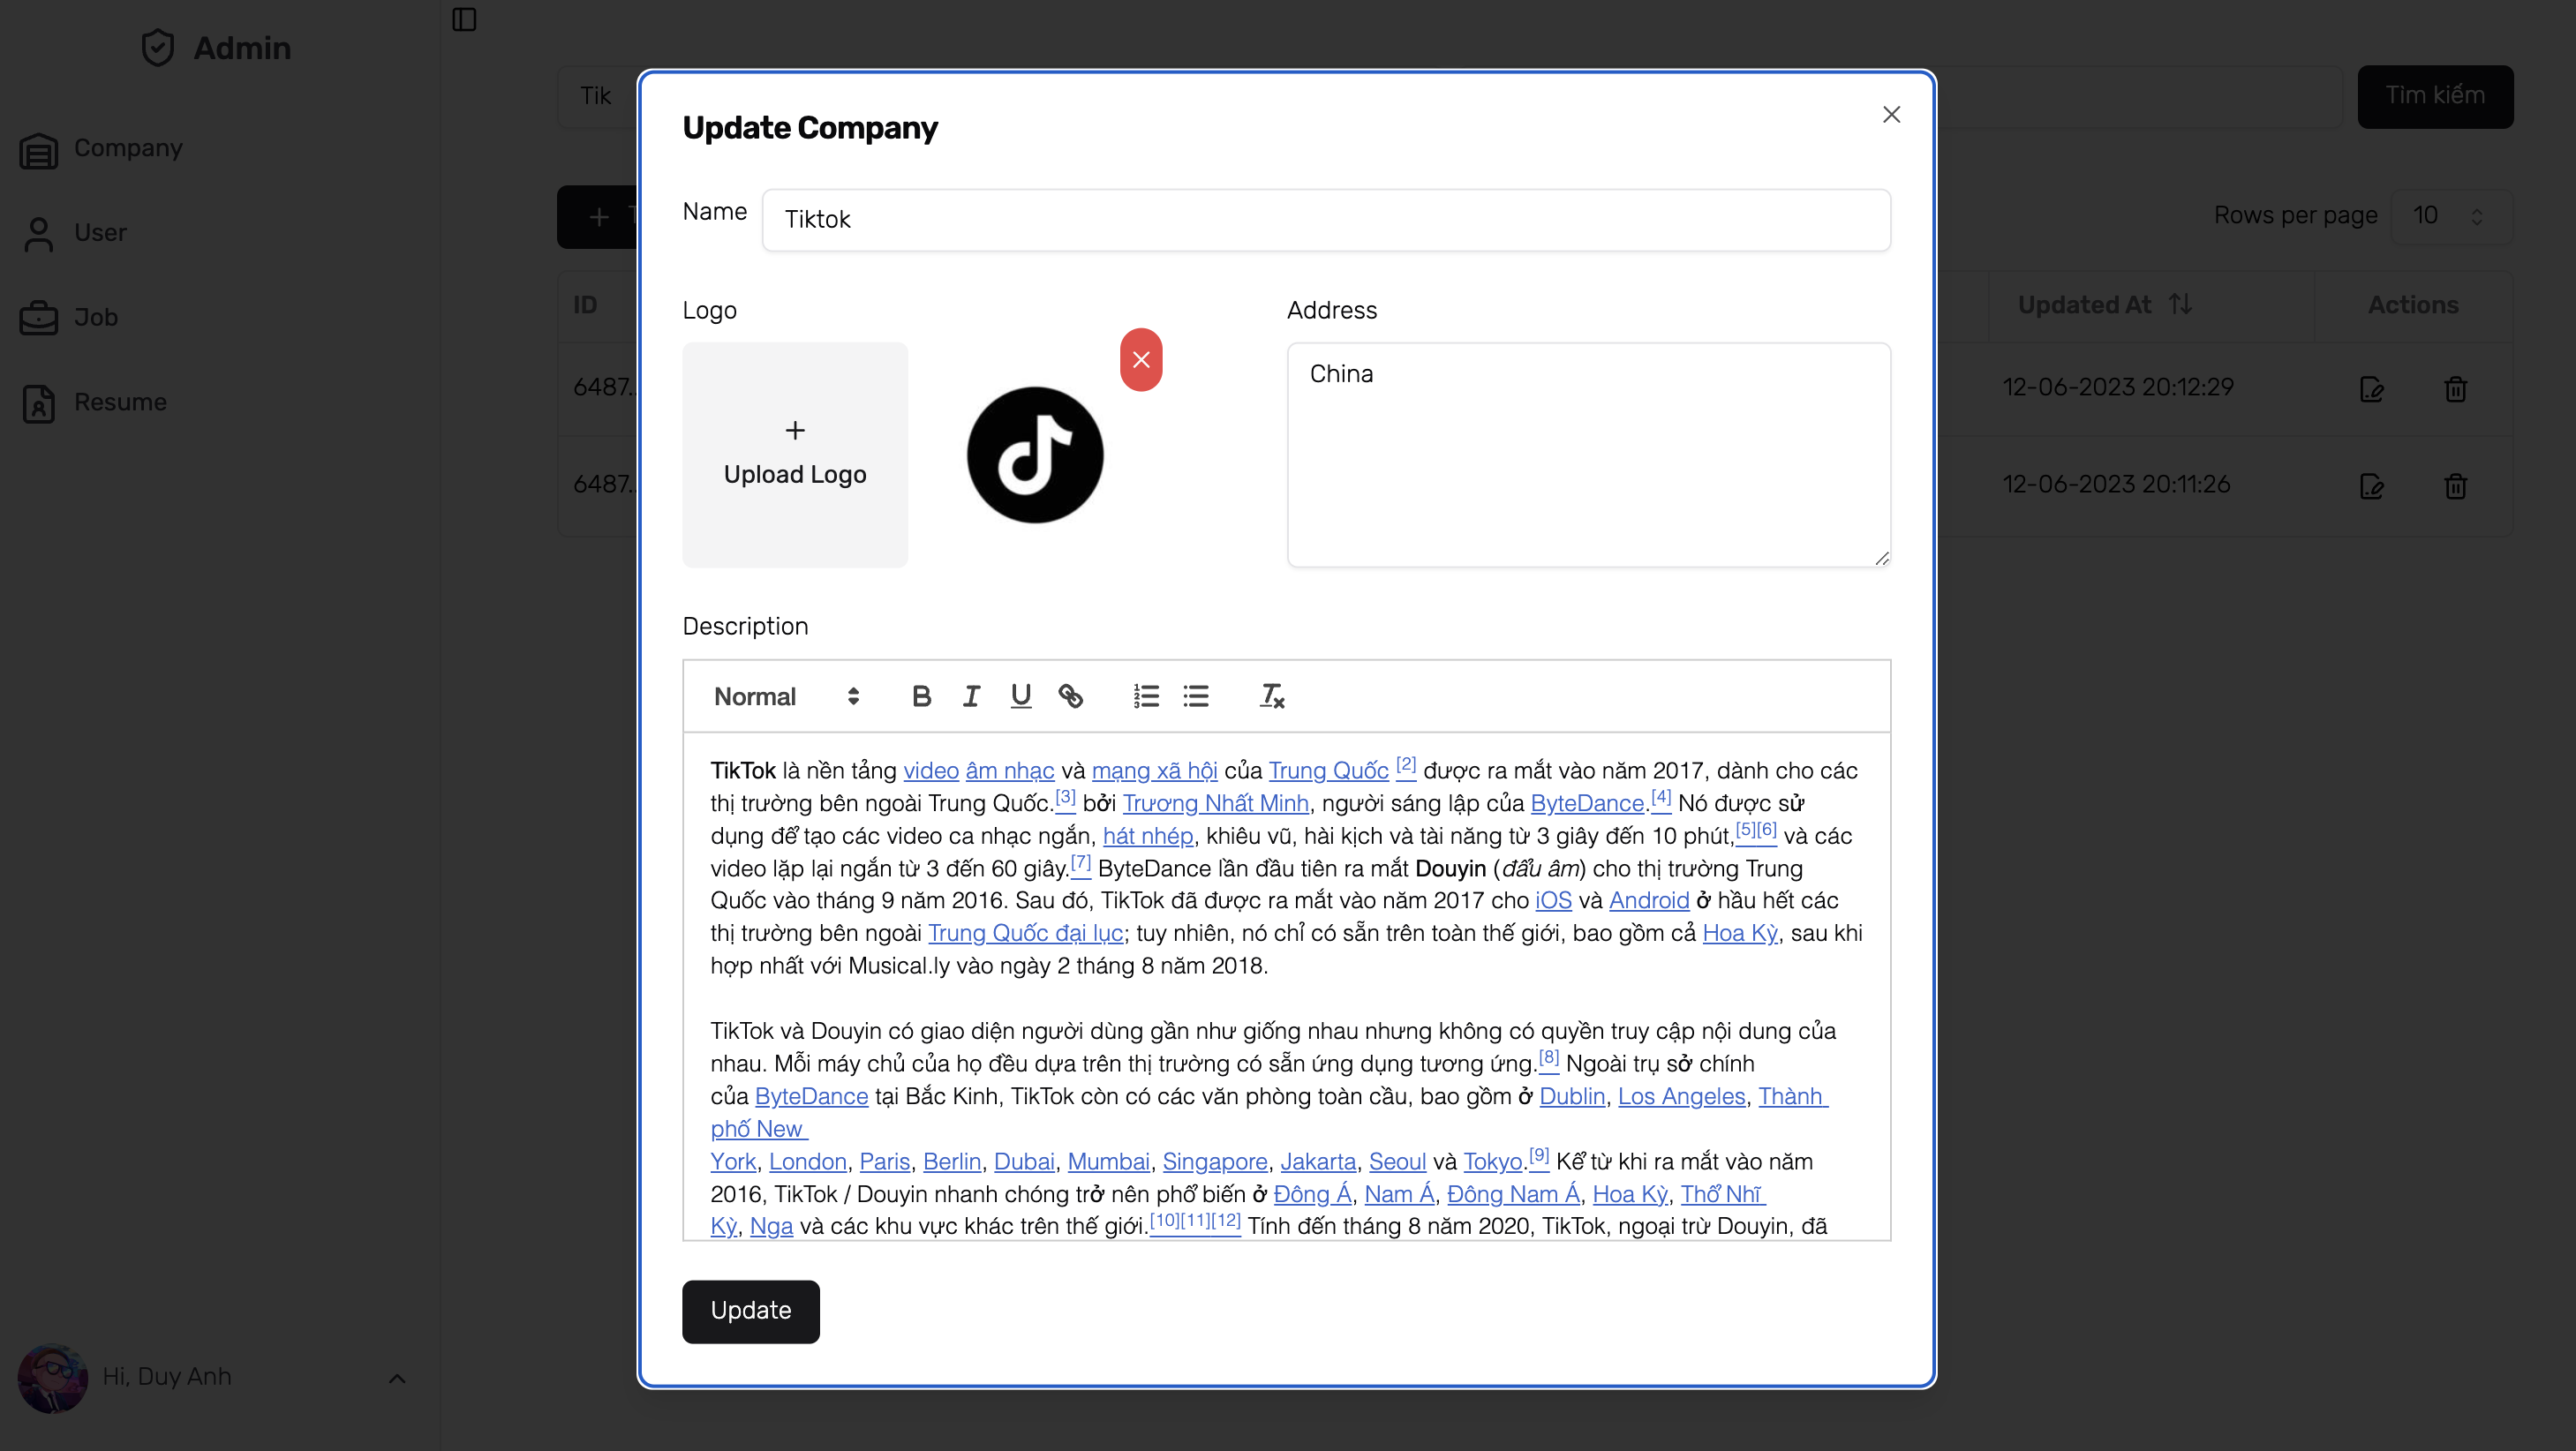
\includegraphics[width=\linewidth]{DBMS-Application/Images/update-company.png}
        \caption{Trang quản lý công ty - Cập nhật thông tin công ty}
        \label{fig:enter-label}
    \end{figure}

    \item \textbf{Delete}: Xoá công ty cụ thể
    \begin{figure}[H]
        \centering
        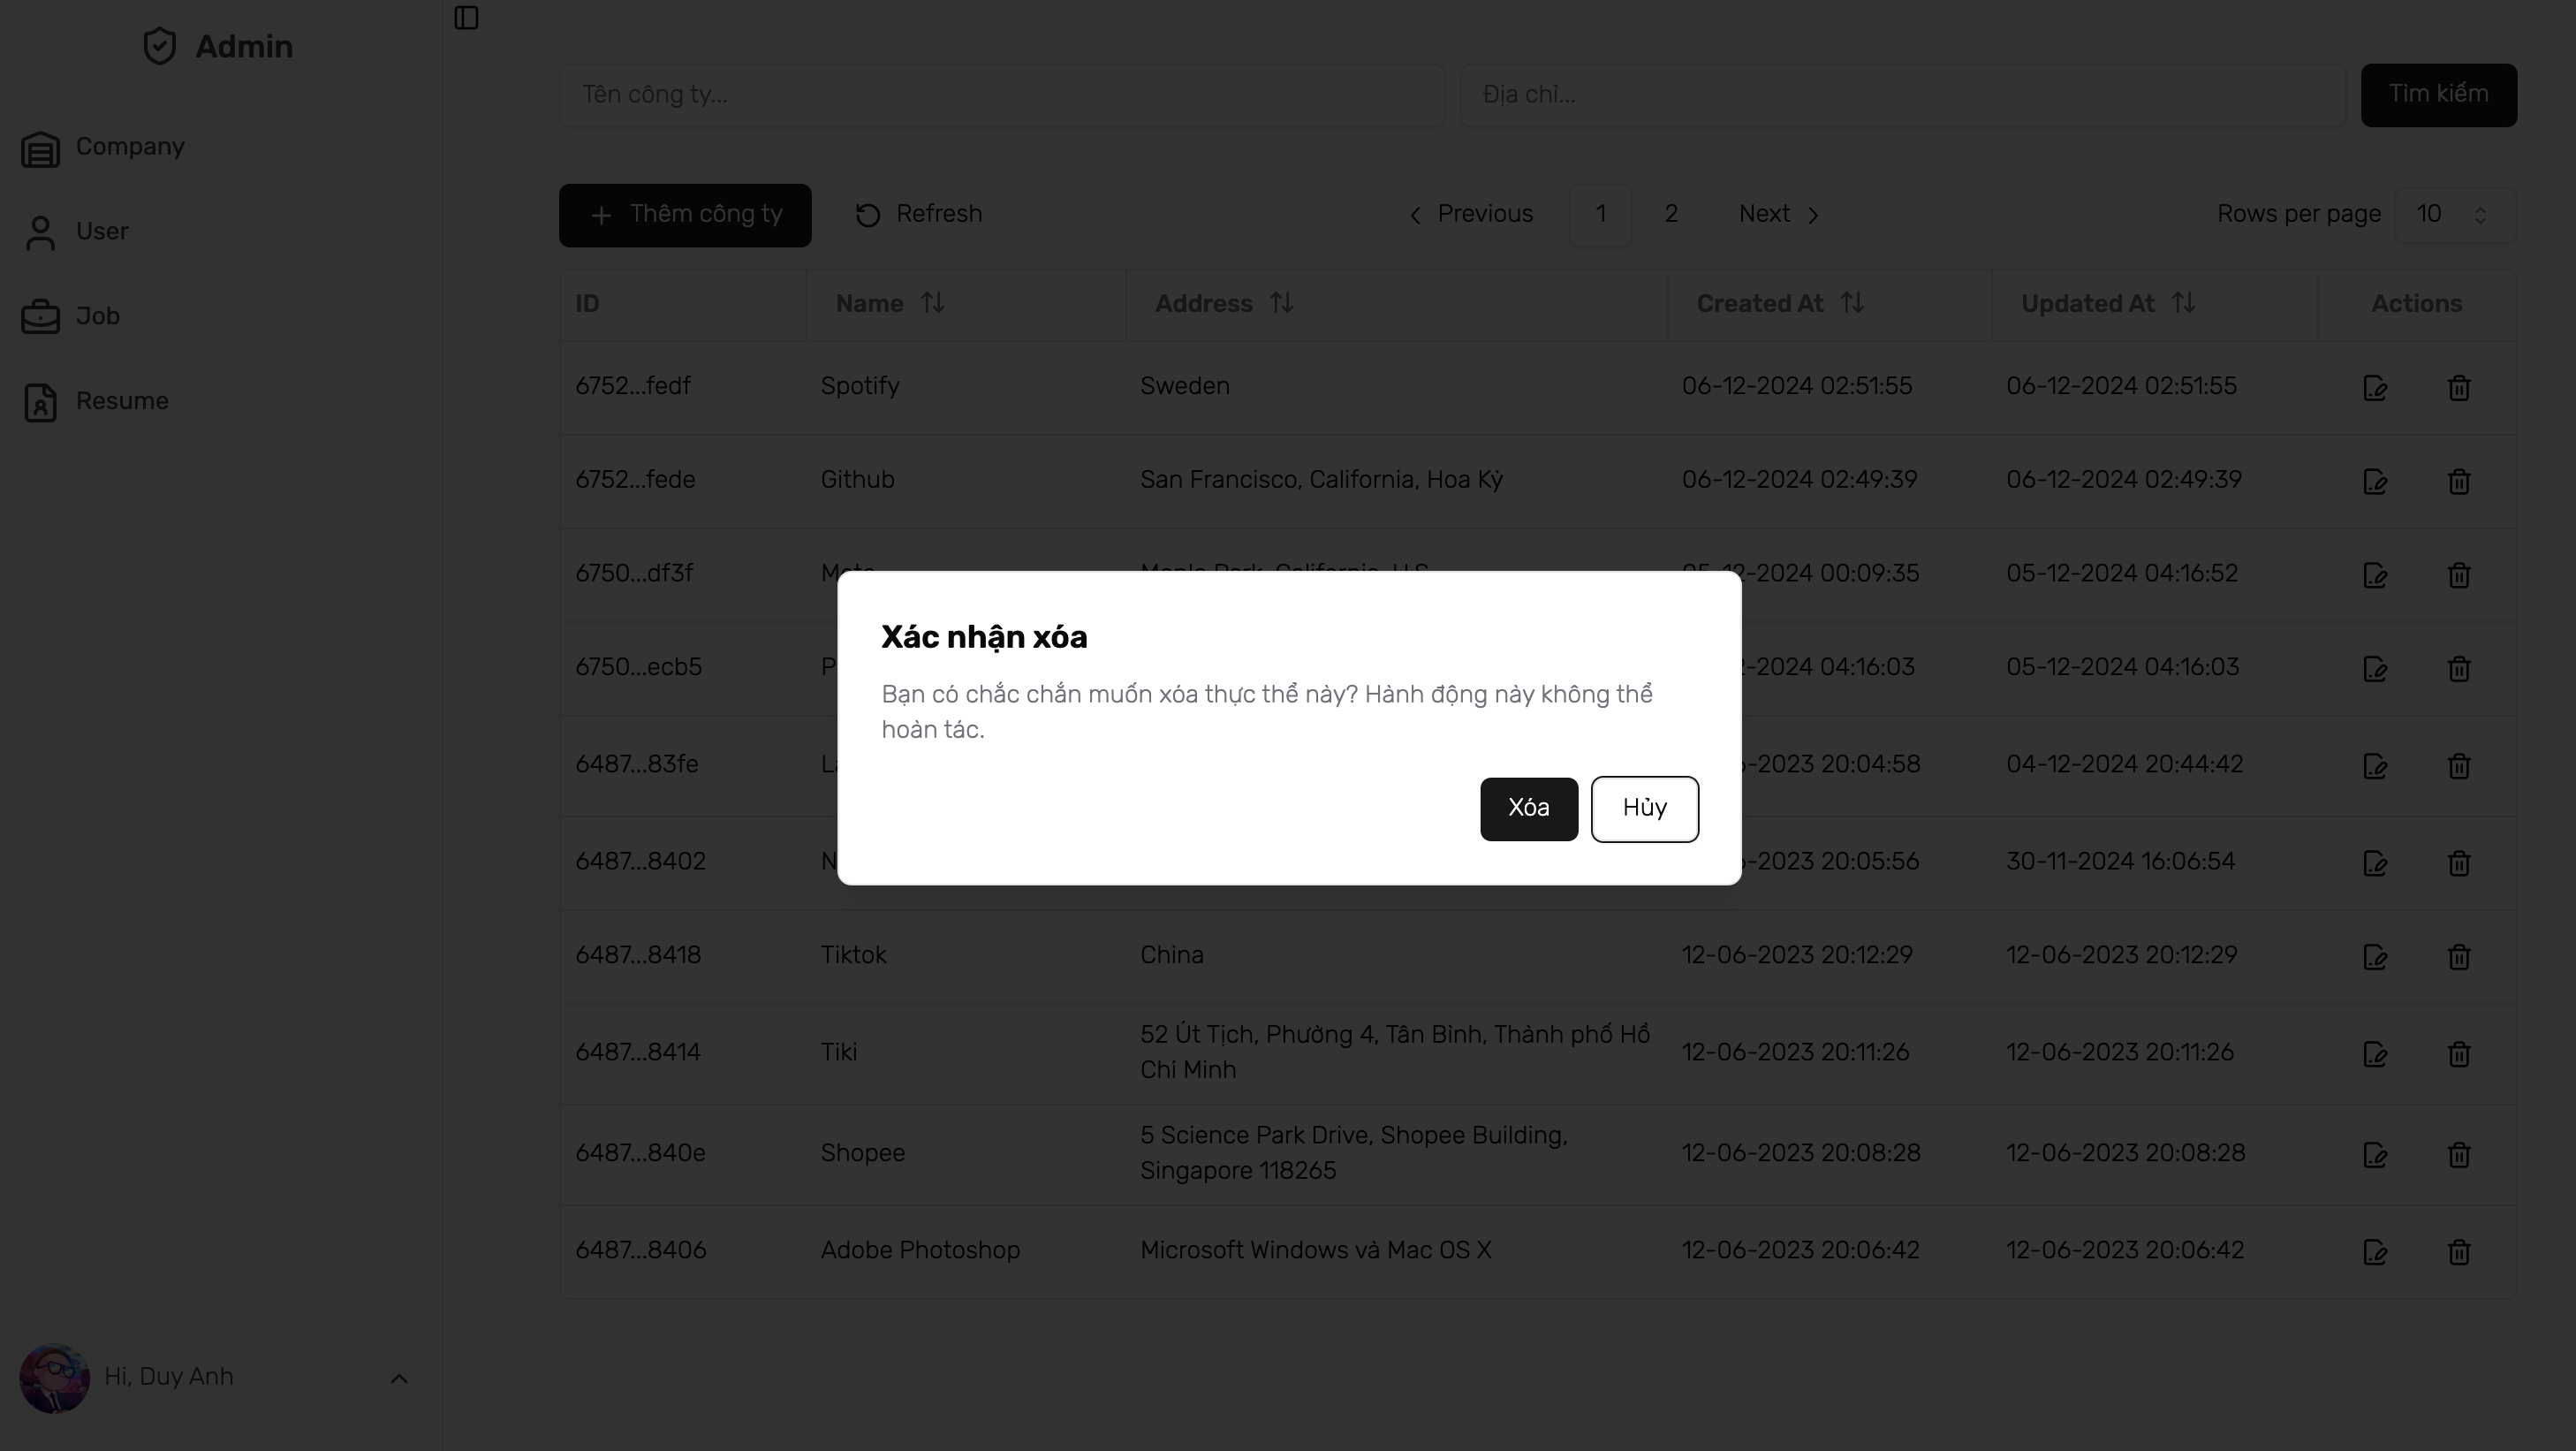
\includegraphics[width=\linewidth]{DBMS-Application/Images/delete-company.png}
        \caption{Trang quản lý công ty - Xoá công ty}
        \label{fig:enter-label}
    \end{figure}
\end{itemize}